%-------------------------------------------------------------------------
\section{Introduction}
\label{sec:intro}

The proliferation of egocentric video content, particularly in instructional domains such as cooking, has created opportunities for developing intelligent assistive systems that help users learn skills, identify mistakes, and receive personalized guidance. However, detecting procedural errors in such videos remains challenging, requiring understanding of both visual observations and their semantic relationship to procedural knowledge encoded in textual instructions.

\begin{figure}[t]
  \centering
  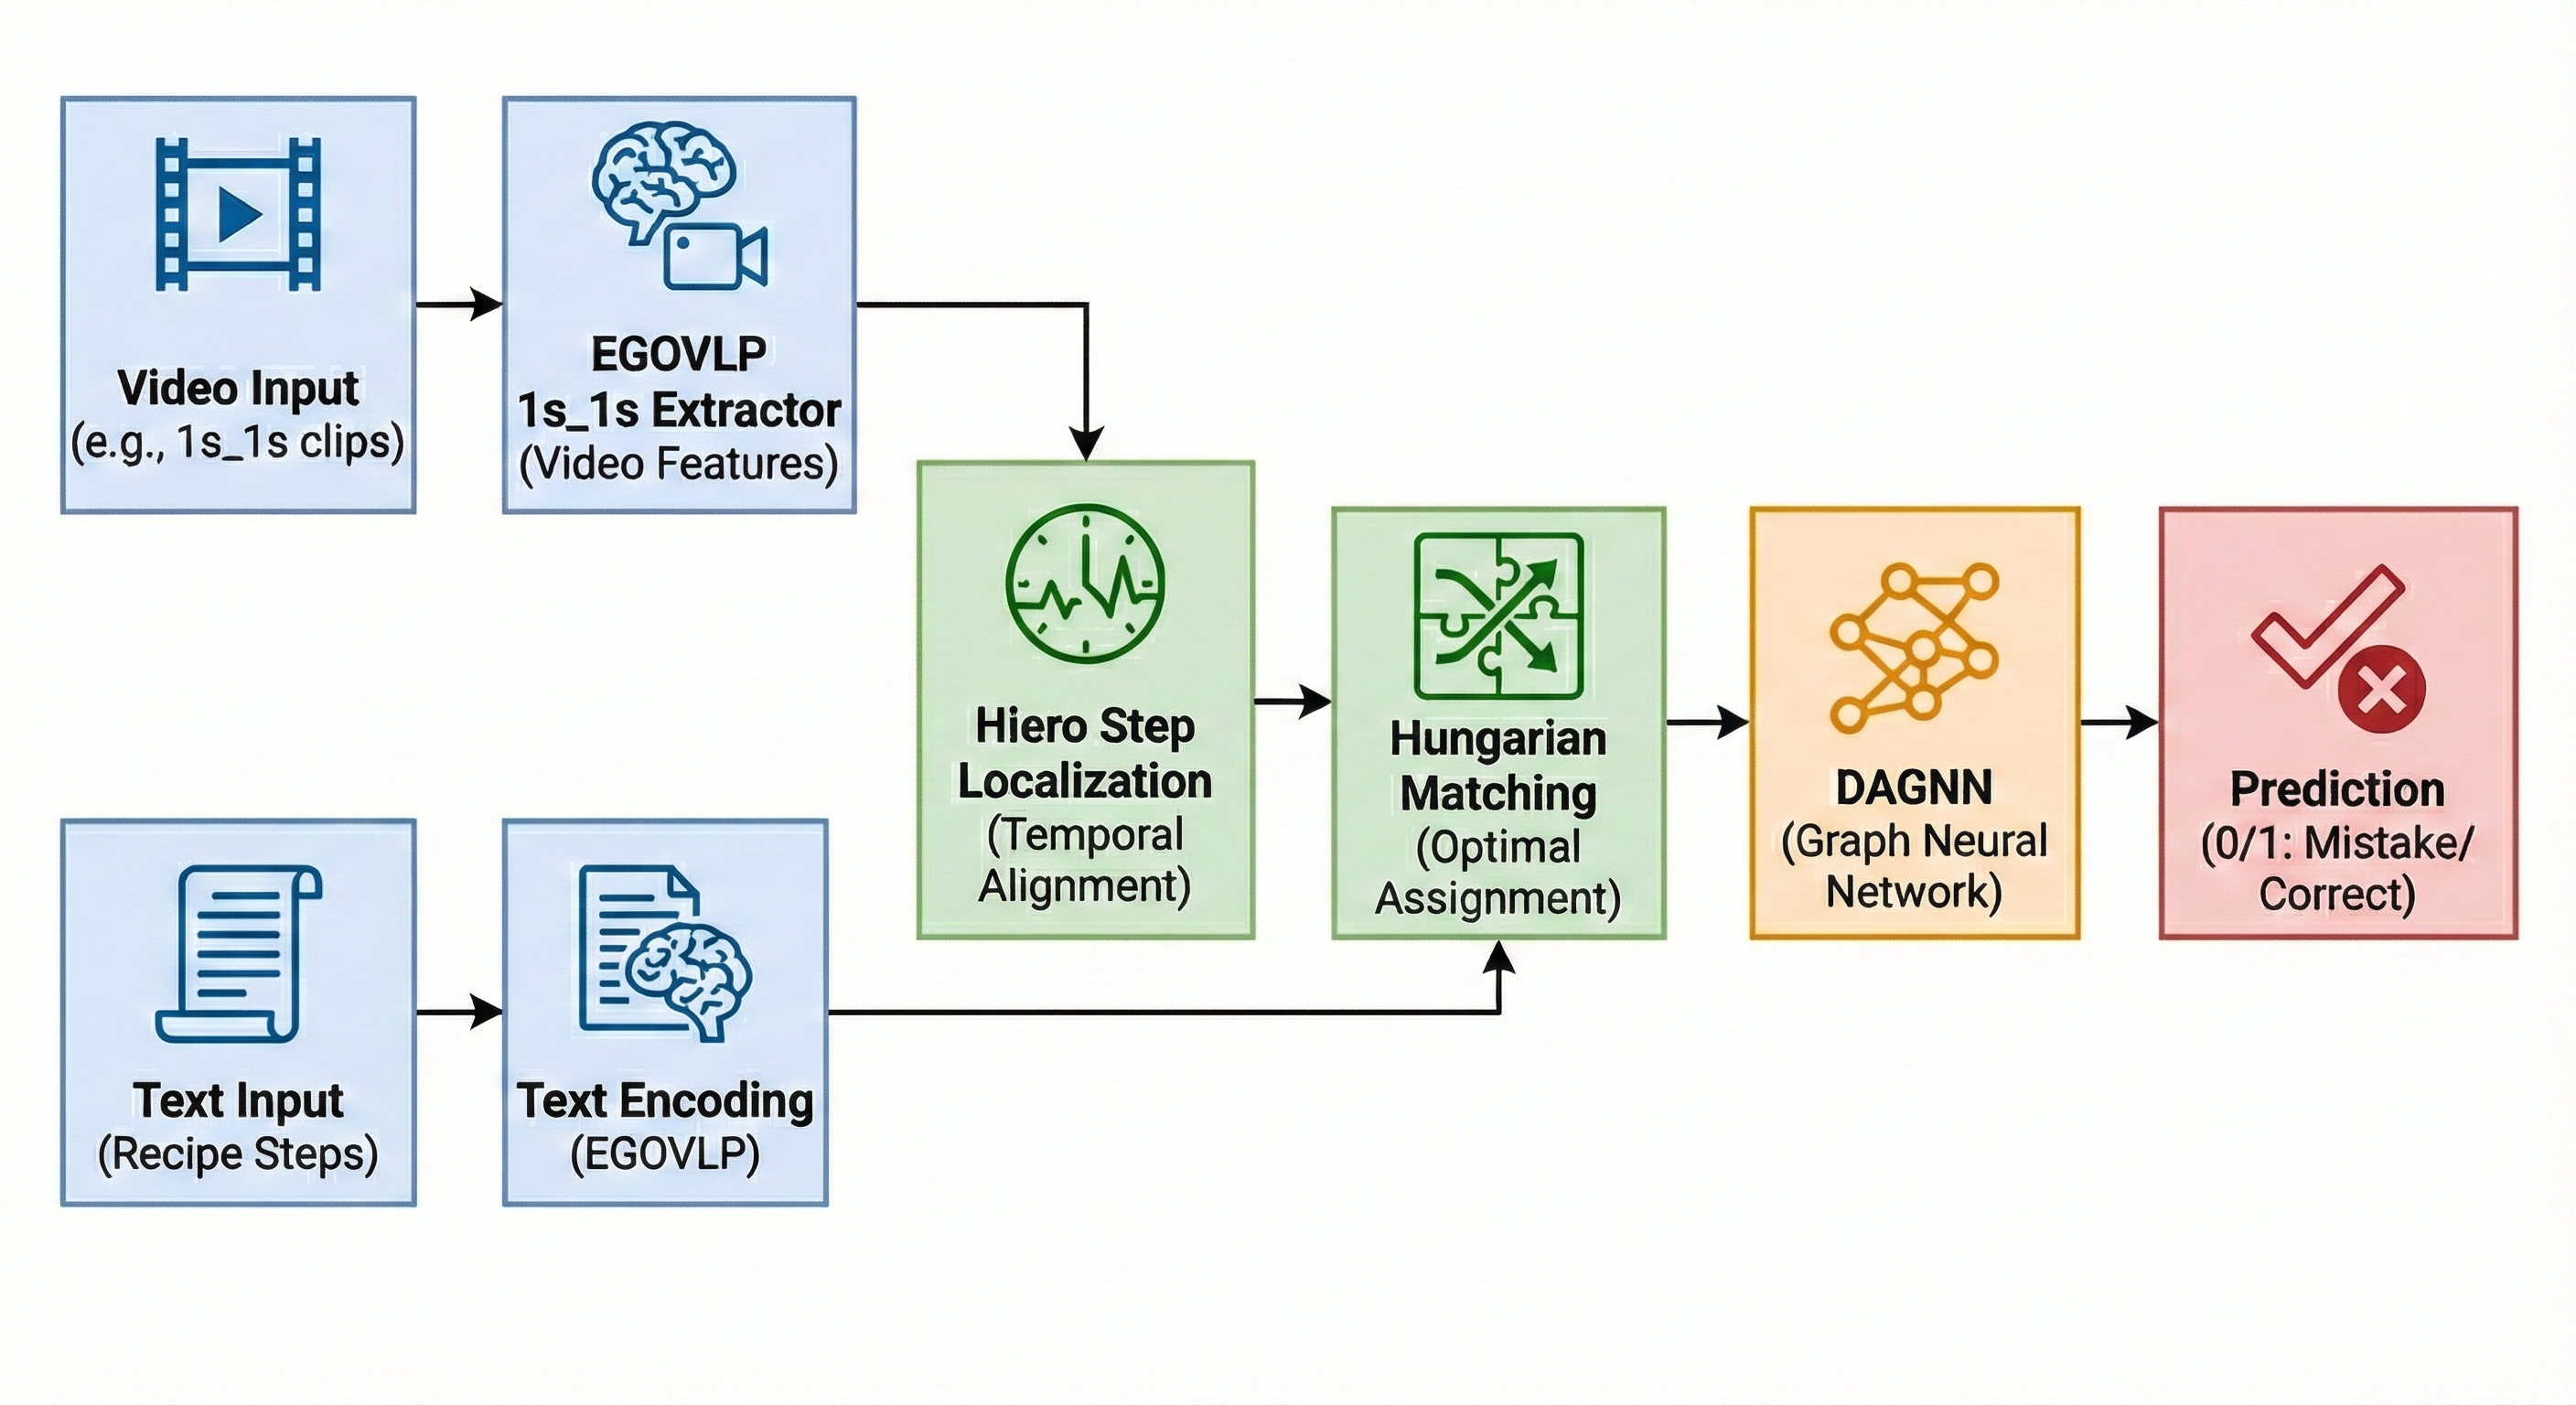
\includegraphics[width=\columnwidth]{figures/figure_1.png}
  \caption{Overview of our procedural error detection framework. We model cooking recipes as directed acyclic graphs and align visual observations from egocentric videos with textual recipe steps using multimodal embeddings.}
  \label{fig:overview}
\end{figure}

Cooking is particularly suitable for studying procedural error detection: recipes naturally form directed acyclic graphs (DAGs) where steps must be executed in specific causal order, and deviations significantly impact outcomes. Moreover, egocentric cooking videos capture the natural first-person perspective of task execution, making them relevant for applications in augmented reality, assistive robotics, and personalized education.

Procedural error detection faces fundamental challenges: (\textit{i}) the \textbf{semantic gap} between low-level visual features and high-level procedural concepts in recipe instructions; (\textit{ii}) the \textbf{temporal alignment problem} requiring correspondences between variable-length observed actions and prescribed recipe steps; (\textit{iii}) the \textbf{causal structure} where actions can only be identified as erroneous within their broader procedural context.

Traditional action recognition approaches classify isolated actions without considering procedural context or textual instructions. While recent egocentric video understanding has progressed in action segmentation and step localization, these methods typically operate in isolation without explicitly modeling structured procedural knowledge.

We propose a graph-based multimodal learning approach using \textbf{Directed Acyclic Graph Neural Networks (DAGNNs)} to model recipe causal structure while integrating visual and textual information at the node level. We use EgoVLP embeddings from video segments and recipe text, aligned through Hungarian matching to establish semantic correspondences. The resulting multimodal graph representation preserves both procedural structure and semantic alignments.

We evaluate on the Captain Cook 4D dataset~\cite{captaincook4d}. Our experiments reveal important insights: despite theoretical soundness, our model achieves modest performance, with analysis identifying two primary limiting factors: (\textit{i}) \textbf{limited dataset size} providing insufficient training examples, and (\textit{ii}) \textbf{zero-shot step localization limitations} from HiERO introducing noise and misalignments in Hungarian matching.

The main contributions of this paper are:
\begin{enumerate}
    \item A graph-based framework for procedural error detection using DAGNNs to model recipe structure while integrating multimodal visual and textual information.
    \item A systematic approach for aligning visual observations with recipe steps using Hungarian matching with explicit handling of unmatched procedural steps or visual observations.
    \item Empirical analysis on Captain Cook 4D revealing limitations of zero-shot weakly supervised approaches.
    \item Transparent discussion of results identifying dataset size and step localization quality as critical bottlenecks.
\end{enumerate}
